% Options for packages loaded elsewhere
\PassOptionsToPackage{unicode}{hyperref}
\PassOptionsToPackage{hyphens}{url}
%
\documentclass[
]{book}
\usepackage{amsmath,amssymb}
\usepackage{iftex}
\ifPDFTeX
  \usepackage[T1]{fontenc}
  \usepackage[utf8]{inputenc}
  \usepackage{textcomp} % provide euro and other symbols
\else % if luatex or xetex
  \usepackage{unicode-math} % this also loads fontspec
  \defaultfontfeatures{Scale=MatchLowercase}
  \defaultfontfeatures[\rmfamily]{Ligatures=TeX,Scale=1}
\fi
\usepackage{lmodern}
\ifPDFTeX\else
  % xetex/luatex font selection
\fi
% Use upquote if available, for straight quotes in verbatim environments
\IfFileExists{upquote.sty}{\usepackage{upquote}}{}
\IfFileExists{microtype.sty}{% use microtype if available
  \usepackage[]{microtype}
  \UseMicrotypeSet[protrusion]{basicmath} % disable protrusion for tt fonts
}{}
\makeatletter
\@ifundefined{KOMAClassName}{% if non-KOMA class
  \IfFileExists{parskip.sty}{%
    \usepackage{parskip}
  }{% else
    \setlength{\parindent}{0pt}
    \setlength{\parskip}{6pt plus 2pt minus 1pt}}
}{% if KOMA class
  \KOMAoptions{parskip=half}}
\makeatother
\usepackage{xcolor}
\usepackage{longtable,booktabs,array}
\usepackage{calc} % for calculating minipage widths
% Correct order of tables after \paragraph or \subparagraph
\usepackage{etoolbox}
\makeatletter
\patchcmd\longtable{\par}{\if@noskipsec\mbox{}\fi\par}{}{}
\makeatother
% Allow footnotes in longtable head/foot
\IfFileExists{footnotehyper.sty}{\usepackage{footnotehyper}}{\usepackage{footnote}}
\makesavenoteenv{longtable}
\usepackage{graphicx}
\makeatletter
\def\maxwidth{\ifdim\Gin@nat@width>\linewidth\linewidth\else\Gin@nat@width\fi}
\def\maxheight{\ifdim\Gin@nat@height>\textheight\textheight\else\Gin@nat@height\fi}
\makeatother
% Scale images if necessary, so that they will not overflow the page
% margins by default, and it is still possible to overwrite the defaults
% using explicit options in \includegraphics[width, height, ...]{}
\setkeys{Gin}{width=\maxwidth,height=\maxheight,keepaspectratio}
% Set default figure placement to htbp
\makeatletter
\def\fps@figure{htbp}
\makeatother
\setlength{\emergencystretch}{3em} % prevent overfull lines
\providecommand{\tightlist}{%
  \setlength{\itemsep}{0pt}\setlength{\parskip}{0pt}}
\setcounter{secnumdepth}{5}
\usepackage{booktabs}
\AtBeginDocument{\renewcommand{\chaptername}{Week}}
\usepackage{amssymb}
\usepackage{amsmath}
\usepackage{titling}
\ifLuaTeX
  \usepackage{selnolig}  % disable illegal ligatures
\fi
\usepackage[]{natbib}
\bibliographystyle{plainnat}
\IfFileExists{bookmark.sty}{\usepackage{bookmark}}{\usepackage{hyperref}}
\IfFileExists{xurl.sty}{\usepackage{xurl}}{} % add URL line breaks if available
\urlstyle{same}
\hypersetup{
  pdftitle={STAT0003 Further Probability and Statistics},
  pdfauthor={Ge Li (Sunny)},
  hidelinks,
  pdfcreator={LaTeX via pandoc}}

\title{STAT0003 Further Probability and Statistics}
\author{Ge Li (Sunny)}
\date{March 15 2023}

\begin{document}
\maketitle

{
\setcounter{tocdepth}{1}
\tableofcontents
}
\chapter*{Preface}\label{preface}
\addcontentsline{toc}{chapter}{Preface}

This document is used to document my assignments and weekly exercises of STAT0003.

\chapter{Exercise Sheet 1}\label{exercise-sheet-1}

\section{Question 1}\label{question-1}

You and your friend are presented with \(7\) boxes. \(3\) of the boxes contain delicious chocolates while other \(4\) are filled with deadly mushrooms (disguised as delicious chocolates). Both of you will need to select a box and eat what is inside, but you need to decide which of you will go first.

\textbf{Question 1.1} In order to increase your chance of eating delicious chocolates, should you choose first or second?\\
\textbf{Solution.} Let \(A\) denote the event of getting chocolate in the first trial.\\
Let \(B\) denote the event of getting chocolate in the second trial.\\
\[P(A) = \frac{3}{7}.\] According to the law of total probabilities: \[P(B) = P(B \mid A)P(A) + P(B \mid A')P(A')\] \[\therefore \ P(B) = \frac{2}{6} \cdot \frac{3}{7} + \frac{3}{6} \cdot \frac{4}{7} = \frac{3}{7}\] \[\therefore \ P(A) = P(B)\]
As a result, the chance of eating delicious chocolates remains the same regardless of choosing to go first or second.

\textbf{Question 1.2} If you choose first, what is the probability that you eat delicious chocolates, given that your friend also does?\\
\textbf{Solution.} \[P(A \mid B) = \frac{P(B \mid A) P(A)}{P(B)} = \frac{\frac{2}{6} \cdot \frac{3}{7}}{\frac{3}{7}} = \frac{1}{3}.\]

\textbf{Question 1.3} How would your answer to (i) change if there were three of you: yourself and two friends? Answer this without doing any mathematics or algebra, perhaps by referring to examples from this module.\\
\textbf{Solution.} The answer would not change. This is the same question as the one discussed duringthe lecture where we tried to calculate the probability of the third ball drawn from an urn with 3 black balls and 4 red balls being a black ball. Essentially, the probability always remains the same regardless of the order.

\section{Question 2}\label{question-2}

A class consists of \(12\) girls and \(16\) boys. Jane is one of the girls and Jonathan is one of the boys.

\textbf{Question 2.1} In how many ways can we make a group of \(2\) girls and \(3\) boys?\\
\[\text{Number of ways} = {16 \choose 3}\cdot{12 \choose 2} = 36960.\]

\textbf{Question 2.2} What is the probability that Jane is not in that group but Jonathan is?\\
\[P(\text{Jonathan without Jane}) = \frac{{15 \choose 2} \cdot {11 \choose 2}}{\text{Number of ways}} = \frac{5}{32}.\]

\textbf{Question 2.3} What is the probability that Jonathan is and Jane is not a group of 5 students selected randomly out of the 28?\\
\textbf{Solution.} Let \(E_1\) denote the event that Jonathan is but Jane is not a group of 5 students randomly selected out of the 28. \[P(E_1) = \frac{{26 \choose 4}}{{28 \choose 5}} = \frac{115}{756}.\]

\textbf{Question 2.4} What is the probability that there are at least \(2\) boys and at least \(1\) girl in a randomly selected group of \(5\) students?\\
\textbf{Solution.} Let \(E_2\) denote the event that there are at least \(2\) boys and at least \(1\) girl in a randomly selected group of \(5\) students. \[P(E_2) = \frac{{16 \choose 2} \cdot {12 \choose 3} + {16 \choose 3} \cdot {12 \choose 2} + {16 \choose 4} \cdot {12 \choose 1}}{{28 \choose 5}} = \frac{85200}{98280} \approx 0.8669.\]

\chapter{Exercise Sheet 2}\label{exercise-sheet-2}

\section{Question 1}\label{question-1-1}

Let \(X\) be a random variable with expectation \(\mu\) and variance \(\sigma^2\). Find the expectation and variance of the random variable \(Y = \frac{X - \mu}{\sigma}\).\\
\textbf{Solution.}
\[\begin{aligned} 
&\textbf{Expectation:} \quad & \mathbb{E}(Y) = \frac{\mathbb{E}(X) - \mu}{\sigma} = 0.\\
&\textbf{Variance:}    \quad & Var(Y) =\frac{\sigma^2}{\sigma^2} = 1. 
\end{aligned}\]

\section{Question 2}\label{question-2-1}

Let \(X\) be a discrete random variable with \(\mathbb{E}(X^2) = 0\).

\textbf{Question 2.1} Show that \(P(X = 0) = 1\).\\
\textbf{Solution.} Since we are given that \[\mathbb{E}(X^2) = \sum_{\text{all }x}x^2 P(X = x) = 0,\] and since both \(x^2\) and \(P(X = x)\) are non-negative values, we can deduce that \(X = 0\) is the only possible circumstance. As a result, \(P(X = 0) = 1\).

\textbf{Question 2.2} What is the \(Var(X)\)?\\
\textbf{Solution.} We need to calculate the expected value of \(X\) first, \[\mathbb{E}(X) = 0.\] We are given that \(\mathbb{E}(X^2) = 0\). As a result, \[Var(X) = \mathbb{E}(X^2) - (\mathbb{E}(X))^2 = 0.\]

\section{Question 3}\label{question-3}

The random variable, \(X\), has the following probability mass function \[p(x) = \frac{c}{x(x+1)} \ \ \ (x = 1,2,3,...)\]

\textbf{Question 3.1} Find the value of the constant \(c\).\\
\textbf{Solution.} \[p(x) = \frac{c}{x(x+1)} = \frac{c}{x} - \frac{c}{x+1}\] Since we know that probability mass function (p(x)) has the property that \(\sum p(x) = 1\), \[\sum_{x=1}^{\infty} p(x) = \lim_{n\to\infty}\sum_{x=1}^{n}(\frac{c}{x} - \frac{c}{x+1}) = \lim_{n\to\infty} (\frac{c}{1} - \frac{c}{2} + \frac{c}{2}  + ...  - \frac{c}{n} + \frac{c}{n} - \frac{c}{n+1}) = 1\] \[\therefore \ \lim_{n\to\infty} c \cdot \frac{n}{n+1} = 1\] \[\therefore \ c = 1\]

\textbf{Question 3.2} Find the cumulative distribution function of \(X\) and sketch both the probability mass function and the cumulative density function.\\
\textbf{Solution.} \[F_X(x) = P(X \leq x) = \sum_{1}^{x} \frac{1}{x} - \frac{1}{x+1} = \frac{x}{x+1}\] \[\begin{aligned}
           F_X(x) = P(X \leq x) = 
           \begin{cases}
        0   &   -\infty < x < 1 \\
        \frac{x}{x+1}   &   1 \leq x < \infty \\
           \end{cases}
         \end{aligned}\]

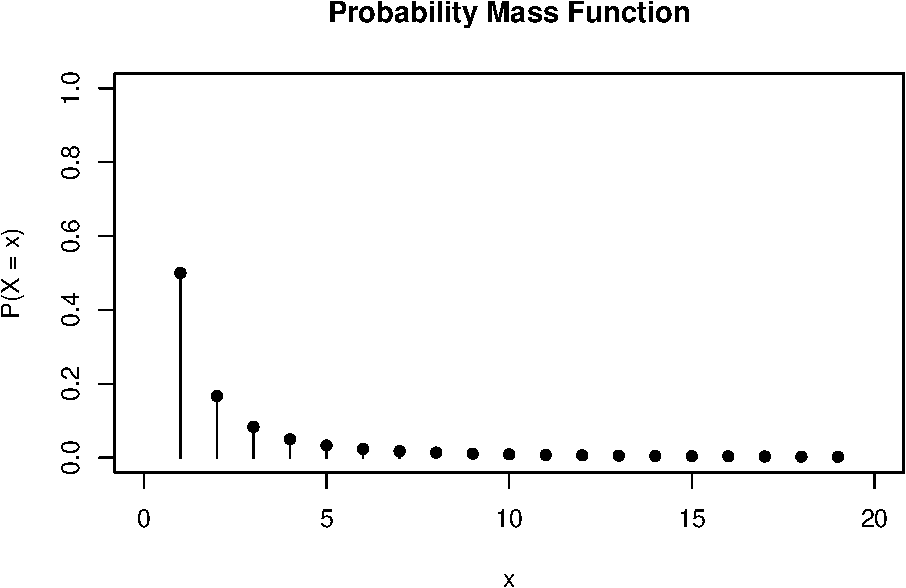
\includegraphics{_main_files/figure-latex/unnamed-chunk-1-1.pdf} 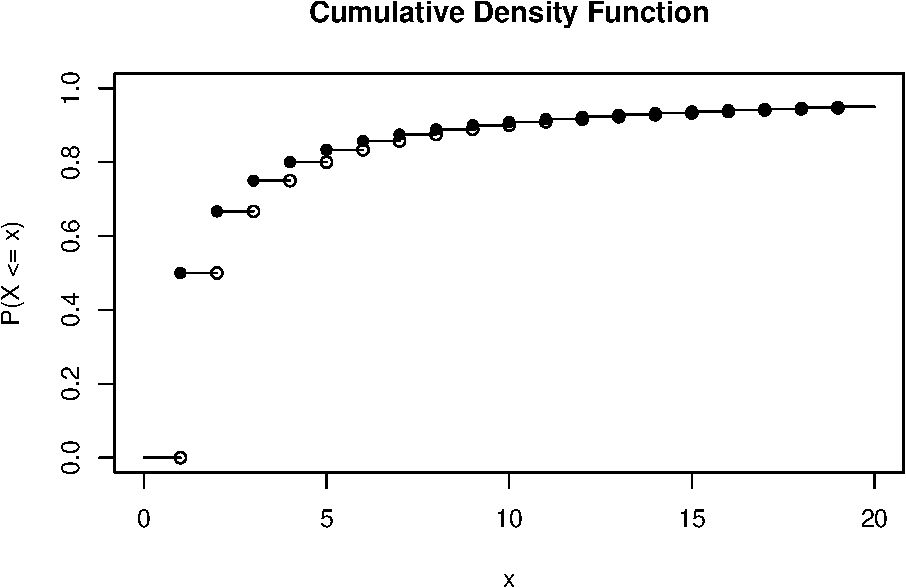
\includegraphics{_main_files/figure-latex/unnamed-chunk-1-2.pdf}

\textbf{Question 3.3} Calculate \(P(X \geq 50)\) and \(P(X \geq 50 \mid X \geq 40)\).\\
\textbf{Solution.}
\[P(X \geq 50) = 1 - P(X < 50) - 1 - P(X \leq 49) = 1 - \frac{49}{50} = \frac{1}{50}\]
\[P(X \geq 50 \mid X \geq 40) = \frac{1/50}{1/40} = \frac{4}{5}\]

\chapter{Exercise Sheet 3}\label{exercise-sheet-3}

\section{Question 1}\label{question-1-2}

A geological study indicates that an exploratory oil well drilled in a certain region should strike oil with probability \(0.3\), independently of other wells drilled. Find the probability that the first strike of oil comes on the third well drilled. Find the probability that the third strike of oil comes on the fifth well drilled.\\
\textbf{Solution.} Let \(X\) denote the number of well drilled until the first strike of oil comes, since then \(X\) follows the distribution \[X \sim \text{geom}(0.3).\] Therefore, the probability that the first strike of oil comes on the third well drilled is \[P(X = 3) = 0.3 \cdot (1-0.3)^2 = 0.147.\]
Let \(M\) denote the event that the third strike of oil comes on the fifth well drilled. The probability of striking oil successfully in the fifth well is \(0.3\), while the probability of having \(2\) wells striking oil successfully in the first \(4\) wells follows a binomial distribution \(\sim \text{bin}(4,0.3)\). Therefore, the probability that the third strike of oil comes on the fifth well drilled is
\[P(M) = \binom{4}{2} \cdot 0.3^2 \cdot 0.7^2 \times 0.3 = 0.07938.\]

\section{Question 2}\label{question-2-2}

An exam paper consists of \(10\) multiple choice questions, each offering \(4\) choices of which only \(1\) (randomly assigned) is correct. If a candidate chooses her answers completely at random, what is the probability of each of the following, specifying the distribution used in each case.

\textbf{Question 2.1} She gets at least \(8\) questions right.\\
\textbf{Solution.} Let \(X\) denote the number of questions the candidate gets correct, as a result, \(X\) follows
\[X \sim \text{bin}(10,0.25).\]
Therefore, the probability the candidate gets at least \(8\) questions right is
\[P(X \geq 8) = \sum_{i = 8}^{10} P(X = i) = \sum_{i=8}^{10} \binom{10}{i} \cdot 0.25^{i} \cdot 0.75^{10-i} = 4.158 \cdot 10^{-4}.\]

\textbf{Question 2.2} The last of the \(10\) questions is the \(8\)th one she gets rights.\\
\textbf{Solution.} Let \(E\) denote the event that the last question being the eighth one the candidate gets right.
The probability of the \(10\)th question being correct is \(0.25\). The probability of the candidate getting \(7\) questions among the first \(9\) questions correct is \(P(X = 7)\), where in this particular case \(X\) follows the distribution \[X \sim \text{bin}(9, 0.25).\]
Therefore, the final probability
\[P(E) = 0.25 \cdot P(X = 7) = 0.25 \times \binom{9}{7} \cdot 0.25^7 \cdot 0.75^2 = 3.090 \cdot 10^{-4}.\]

\textbf{Question 2.3} In \(6\) such exams, she gets at least \(8\) questions right in at most one exam.\\
\textbf{Solution.} Let \(A\) denote the number of exams the candidate gets at least \(8\) questions correct among the \(6\) exams, \(A\) follows the distribution \[A \sim \text{bin}(6, 4.158 \cdot 10^{-4}).\] As a result, \[P(X \leq 1) = \sum_{i=0}^{1} \binom{6}{i} \cdot (4.158 \cdot 10^{-4})^i \cdot (1 - 4.158 \cdot 10^{-4})^{6-i} = 0.9999974.\]

\textbf{Question 2.4} She is told that in one exam, \(6\) of the answers (at random) are given by the same unknown choice. What is the probability that in her first \(4\) answers the candidate chooses \(3\) from that set of \(6\).\\
\textbf{Solution.} The event that the candidate chooses 3 from that set of \(6\) answers in her first 4 answers follows the hypergeometric distribution \(\sim \text{Hypergeometric}(10, 3, 6).\)
\[P = \frac{\binom{4}{3} \cdot \binom{6}{3}}{\binom{10}{6}} = 0.3810.\]

\section{Question 3}\label{question-3-1}

Let \(X \sim \text{Poi}(\mu)\). Prove that \(\mathbb{E}(X) = \mathbb{Var}(X) = \mu\).\\
\[\mathbb{E}(X) = \sum_{\text{all x}} x \cdot \frac{e^{-\mu} \cdot \mu^x}{x!} = \mu e^{-\mu} \sum_{\text{all x}} \frac{\mu^{x-1}}{(x-1)!}\] Since we can identify that \(\sum_{\text{all x}} \frac{\mu^{x-1}}{(x-1)!}\) is the expansion of \(e^{\mu}\),
\[\mathbb{E}(X) = \mu e^{-\mu} \cdot e^{\mu} = \mu.\]
In order to calculate the variance \(\mathbb{Var}(X)\), we need to first calculate the expectation of \(X^2\),
\[\begin{aligned}
\mathbb{E}(X^2) &= \sum_{\text{all x}} x^2 \cdot \frac{e^{-\mu} \cdot \mu^x}{x!} \\
&= \mu e^{-\mu}  \cdot \sum_{\text{all x}} \frac{\mu^{x-1}}{(x-1)!} \cdot [(x-1)+1] \\
&= \mu e^{-\mu} \cdot (\mu \sum_{\text{all x}} \frac{\mu^{x-2}}{(x-2)!} + \sum_{\text{all x}} \frac{\mu^{x-1}}{(x-1)!}) \\
&= \mu e^{-\mu} \cdot (\mu e^{\mu} + e^{\mu}) \\[0.5em]
&= \mu^2 + \mu.
\end{aligned}\]
Therefore, the variance of \(X\) is
\[\mathbb{Var}(X) = \mathbb{E}(X^2) - [\mathbb{E}(X)]^2 = \mu^2 + \mu - \mu^2 = \mu\]
As a result, we have proved that \(\mathbb{E}(X) = \mathbb{Var}(X) = \mu\).

\chapter{Exercise Sheet 4}\label{exercise-sheet-4}

\section{Question 1}\label{question-1-3}

Trains arrive at a station with a mean rate of \(3\) trains/hour: assume that they are arriving from a Poisson Process. Compute the following probabilities (making sure that you clearly define the random variables you are using in each case). You may only use R or a calculator for the exponential function (not for any probability distributions):

\textbf{Question 1.1} If we record the number of trains for \(3\) hours, there are more than \(5\).\\
\textbf{Solution.} Let \(X\) denote the number of trains arriving in \(3\) hours.
\[X \sim \text{pois}(9)\]
\[P(X > 5) = 1 - \sum_{n = 0}^{5} \frac{e^{-9} \cdot 9^n}{n!} = 0.8843\]

\textbf{Question 1.2} If we go to the station and wait for the first train to arrive, then we will not wait more than 10 minutes.\\
\textbf{Solution.} Let \(T\) denote the time passengers wait for the train to arrive.
\[T \sim \text{exp}(3)\]
\[P(T \leq 1/6) = 1 - (1-e^{-3(1/6)}) = 0.3934\]
\textbf{Question 1.3} If we go to the station and take the third train that comes, we will not wait more than 30 minutes. Evaluate the integral by repeated integration by parts.\\
\textbf{Solution.} \[T \sim \text{gamma}(\text{shape} = 3, \text{rate} = 3/2)\]
\[\begin{aligned}
P(T \leq 1) &= \int_0^1 \frac{(3/2)^3x^2 e^{-3x/2}}{2!} \,dx = \frac{27}{16} \int_0^1 x^2 e^{-3x/2} \,dx \\
&= \frac{27}{16}\bigg[x^2(-2/3)e^{-3x/2}\bigg]_0^1 - \frac{27}{16} \int_0^1 (-\frac{4}{3}xe^{-3x/2}) \,dx \\
&= \frac{27}{16}(-2e^{-3/2}/3 - \frac{40}{27}e^{-3/2} + \frac{16}{27}) \\[0.3em]
&\approx 0.1912
\end{aligned}\]
We can confirm this answer by using \emph{pgamma(1,3,3/2)}.
These are not sensible assumptions, considering the fact that trains don't arrive at stations at randomly chosen time, and the time of arrivals of each train may not necessarily be independent.

\section{Question 2}\label{question-2-3}

The probability density function of \(X\), the lifetime in hours of a certain type of electronic device is given by
\[f(x) = \begin{cases} 10/x^2 & x > c \\ 0 & \text{otherwise} \end{cases}\]
Find \(c\) and \(P(X > 15)\). What is the probability that out of \(5\) such devices at least \(4\) will function for at least \(15\) hours (assume the lifetimes of the devices are independent)?\\
\textbf{Solution.} \[F_X(x) = \int_{x=c}^{\infty} \frac{10}{x^2} \,dx = 1\]
\[\therefore \ \bigg[-\frac{10}{x} \bigg]_c^\infty = 1\]
\[\therefore \ c = 10\]
\[P(X > 15) = \int_{15}^{\infty} \frac{10}{x^2} \,dx = \bigg[-\frac{10}{x} \bigg]_{15}^\infty = \frac{2}{3}\]
Let M denote the number of the electronic devices that function well for at least \(15\) hours.
\[M \sim \text{binom}(5, \frac{2}{3})\]
\[P(M \geq 4) = \binom{5}{4}\bigg(\frac{2}{3}\bigg)^4\bigg(\frac{1}{3}\bigg)^1 + \binom{5}{5}\bigg(\frac{2}{3}\bigg)^5 = 0.4609\]

\section{Question 3}\label{question-3-2}

\textbf{Question 3.1} The mean of a \(\text{Gamma}(\alpha, \lambda)\) distribution.\\
\textbf{Solution.} Since we are given that
\[\int_{0}^{\infty} \frac{x^{\alpha-1} e^{-\lambda x} \lambda^\alpha}{\Gamma(\alpha)} \,dx = 1.\]
\[\begin{aligned}
\mathbb{E}(X) &= \int_{0}^{\infty} x \cdot \frac{x^{\alpha-1}e^{-\lambda x} \lambda^\alpha}{\Gamma(\alpha)} \,dx \\
&= \int_{0}^{\infty} \frac{x^{\alpha}e^{-\lambda x} \lambda^{\alpha+1}}{\lambda \cdot \Gamma(\alpha)} \,dx \\
&= \frac{\alpha}{\lambda} \int_{0}^{\infty}  \frac{x^{\alpha} e^{-\lambda x} \lambda^{\alpha+1}}{\Gamma(\alpha+1)} \,dx \\
&= \frac{\alpha}{\lambda}
\end{aligned}\]

\textbf{Question 3.2} Find the result of \(\int_0^{\infty} x^2 e^{-cx} \,dx\).\\
\textbf{Solution.} \[\Gamma(3) = \int_0^{\infty} x^2 e^{-cx} \,dx\]
We use substitution, let \(u = cx\), then \(dx = \frac{1}{c}du\).
\[\int_0^{\infty} x^2 e^{-cx} \,dx = \frac{1}{c^3} \int_{0}^{\infty} u^2 e^{-u} \,du = \frac{2}{c^3}\]

\textbf{Question 3.3} Derive the Mean and Variance of continuous r.v. \(X\), whose pdf is \(\frac{a}{2}e^{-a|x|}\) over the real line.\\
\textbf{Solution.}\\
\[\begin{aligned}
\mathbb{E}(X) &= \int_{-\infty}^{\infty} \frac{ax}{2}e^{-a|x|} \,dx \\
&= \frac{1}{2} \bigg(\int_{-\infty}^{0} axe^{-ax} \,dx + \int_{0}^{\infty} axe^{-ax} \,dx \bigg) \\
&= 0
\end{aligned}\]
\[\begin{aligned}
\mathbb{E}(X^2) &= \int_{-\infty}^{\infty} \frac{ax^2}{2}e^{-a|x|} \,dx \\
&= \int_{0}^{\infty} ax^2e^{-ax} \,dx \\
&= a \int_{0}^{\infty} x^2 e^{-ax} \,dx \\
&= a \cdot \frac{2}{a^3} \ \text{(according to (b))} \\
&= \frac{2}{a^2}
\end{aligned}\]
As a result, the variance is \[\mathbb{Var} = \frac{2}{a^2}.\]

\chapter{Exercise Sheet 5}\label{exercise-sheet-5}

\section{Question 1}\label{question-1-4}

The annual rainfall in inches in a certain region is modelled by a normal random variable with mean \(40\) and variance \(16\) What is the probability that it will take at least \(5\) years until a year occurs having a rainfall of over \(45\) inches? What assumptions are you making?\\
\textbf{Solution.} Assumption: annual rainfall of each year is independent.\\
Let \(X\) denote the annual rainfall in inches in that certain region. \[X \sim \text{norm}(40, 16)\]
Therefore, the probability of a year having a rainfall of over \(45\) inches is \[P(X > 45) = 1 - P(X \leq 45) = 1 - \Phi \bigg(\frac{45-40}{4}\bigg) = 1 - 0.8944 = 0.1056.\] Alternatively, we can use the R command \texttt{pnorm(45,\ 40,\ 4,\ lower.tail\ =\ F)} to find the probability. Let \(Y\) denote the number of years until a year occurs having a rainfall of over \(45\) inches. Therefore, \(Y\) follows the geometric distribution \[Y \sim \text{geom}(0.1056).\]
The probability that it takes at least \(5\) years until a year occurs having a rainfall of over \(45\) inches is
\[P(Y \geq 5) = 1 - P(Y \leq 4) = 1 - (1 - (1 - 0.1056)^4) = 0.6399.\] Alternatively, we can use the R command \texttt{pgeom(3,\ 0.1056,\ lower.tail\ =\ F)} to find the probability.

\section{Question 2}\label{question-2-4}

Assume that \(X_1, ..., X_{10}\) are independent normally distributed random variables, each with mean \(5\) and variance \(1\).\\
\textbf{Question 2.1} Find the probability that \(X_i > 5\) for all \(i = 1,...,10\).\\
\textbf{Solution.} For all \(X_1, ..., X_{10}\), the probability of \(X_i > 5\) is
\[P(X_i > 5) = 1 - P(X_i \leq 5) = 1 - \Phi(0) = 0.5.\]

\textbf{Question 2.2} Find the probability that at least two of the \(X_i\)s are greater than \(5\).\\
\textbf{Solution.} Let \(A\) denote the number of \(X_i\)s that are greater than \(5\). Since then, \(A\) follows the binomial distribution
\(A \sim \text{binom}(10, 0.5)\).
\[P(A \geq 2) = 1 - P(A \leq 1) = 1 - \binom{10}{0} \cdot 0.5^{10} - \binom{10}{1} \cdot 0.5^{10} = 0.9893.\]

\textbf{Question 2.3} Find the probability that the sample mean of the \(X_i\)s is greater than \(5.1\).\\
\textbf{Solution.} For \(X_1, ..., X_{10}\) that are independent normally distributed random variables with mean \(5\) and variance \(1\), the sample mean of \(X_i\)s is normally distributed with mean \(5\), and variance \(\frac{1}{10}\).
\[P(\bar{X} > 5.1) = 1 - P(\bar{X} \leq 5.1) = 1 - \Phi\bigg(\frac{5.1-5}{\sqrt{1/10}}\bigg) = 1 - 0.6255 = 0.3745,\]
R command \texttt{pnorm(5.1,\ 5,\ sqrt(1/10),\ lower.tail\ =\ F)} returns \(P(\bar{X} > 5.1) = 0.3759\).

\textbf{Question 2.4} Without doing any further calculations, write down the probability that the sum of all the \(X_i\)s is greater than \(51\). Why were no further calculations necessary?\\
\textbf{Solution.} The probability that the sum of all the \(X_i\)s is greater than \(51\) is the same as the probability that the sample mean of the \(X_i\)s is greater than \(5.1\) since if the sample mean is greater than \(5.1\), the sum would definitely be greater than \(51\).
\[\therefore \ P \bigg(\sum_{i=1}^{10} X_i > 51 \bigg) = P(\bar{X} > 5.1) = 0.3745 \ \text{or} \ 0.3759.\]

\chapter{Exercise Sheet 6}\label{exercise-sheet-6}

\section{Question 1}\label{question-1-5}

Here are the weights of some rather greedy dogs (in kgs): \(39.6 \ 40.2 \ 40.9 \ 41.4 \ 39.8 \ 39.4 \ 43.6 \ 41.8 \ 40.9\).\\
\textbf{Question 1.1} Assuming a Normal model for the population of such dogs, calculate the \(92\%\) confidence interval for \(\mu\) and interpret this in words.\\
\textbf{Solution.} Let \(X\) denote the weights of the dogs. We first compute the sample mean and sample variance of the data.
\[\bar{X} = \frac{\sum X_i}{n} = \frac{1}{9} \cdot (39.6+40.2+40.9+41.4+39.8+39.4+43.6+41.8+40.9) = 40.84\]
\[\because \ S^2 = \frac{\sum (X_i - \bar{X})^2}{n-1} = \frac{\sum X_i^2 - 2\bar{X}\sum X_i + n\bar{X}^2}{n-1} = \frac{\sum X_i^2 - n \bar{X}^2}{n-1}\]
\[\therefore \ S^2 = \frac{39.6^2 + 40.2^2 + 40.9^2 + 41.4^2 + 39.8^2 + 39.4^2 + 43.6^2 + 41.8^2 + 40.9^2 - 9 \cdot \bar{X}^2}{9-1} = 1.75\]
Consider the pivotal quantity
\[T = \frac{\sqrt{n}(\bar{X}-\mu)}{S} \ \dot\sim \ \text{t}(\text{df} = n-1).\]
\[\because \ P \bigg(t_{\alpha/2} < \frac{\sqrt{n}(\bar{X}-\mu)}{S} < t_{1-\alpha/2} \bigg) = 1 - \alpha\]
\[\therefore P \bigg(\bar{X} - t_{1-\frac{\alpha}{2}} \frac{S}{\sqrt{n}} < \mu < \bar{X} + t_{1-\frac{\alpha}{2}} \frac{S}{\sqrt{n}} \bigg) = 1 - \alpha\]
As a result, the \((1-\alpha) \cdot 100\%\) confidence interval for \(\mu\) is
\[\bigg(\bar{X} - t_{1-\frac{\alpha}{2}} \frac{S}{\sqrt{n}}, \ \bar{X} + t_{1-\frac{\alpha}{2}} \frac{S}{\sqrt{n}} \bigg)\]
In this case, since we are required to find the \(92\%\) confidence interval for \(\mu\), we take \(\alpha = 0.08\) as the confidence coefficient. We compute \(t_{8, 0.96}\) using the R command \texttt{qt(0.96,\ df\ =\ 8)} which returns \(t_{8, 0.96} = 2.00\).
Therefore, the \(92\%\) confidence interval for \(\mu\) is
\[\bigg( 40.84 - 2 \cdot  \frac{\sqrt{1.75}}{3}, \ 40.84 + 2 \cdot  \frac{\sqrt{1.75}}{3} \bigg) = (39.96, 41.72).\]
This represents that we are \(92\%\) confident that the population mean of the weights of the dogs is between the range \(39.96\) and \(41.72\).

\textbf{Question 1.2} What caused the difference in confidence interval for \(\mu\) in \(2\) exercises?\\
\textbf{Solution.} The difference in confidence interval for \(\mu\) is caused by different distributions we used to approximate the random variables. In last exercise, we used Standard Normal Distribution instead of Student T Distribution since the population variance were known and given to us (\(\sigma^2 = 2\)). Note that the reason of one of the confidence intervals being wider than the another is that T Distribution has fatter tails and therefore has larger quantiles, which evantually lead to a wider confidence interval.

\section{Question 2}\label{question-2-5}

We decide to model cars entering a motorway service station with a Poisson Process of rate \(1500\) / day.\\
\textbf{Question 2.1} Which exact distribution would we use to model the total number of cars that enter
during June?\\
\textbf{Solution.} We should use Poisson Distribution. Let \(Y\) denote the number of cars entering the motorway service station every day. According to what we are given, \(Y \sim \text{Pois}(1500)\). Then, let \(X\) denote the number of cars entering the motorway service station in June, which is a 30-day period, \(X\) follows the Poisson Distribution \(X \sim \text{Pois}(45000)\).

\textbf{Question 2.2} Use the CLT to calculate the probability that greater than \(44800\) but less than \(45200\) cars entered during June, defining the appropriate random variables formally. Are the conditions for the CLT satisfied?\\
\textbf{Solution.} Let \(X\) denote the total number of cars entering the service station in June. We can consider \(X\) as the sum of \(30\) I.I.D random variables with mean and variance \(\mu = \sigma^2 = 1500\). Therefore, we can approximate \[X \dot\sim N(30\cdot 1500, 30\cdot 1500) = N(45000, 45000).\]
As a result, the probability that greater than \(44800\) but less than \(45200\) cars entered during June is
\[P(44800 - 0.5 < X < 45200 + 0.5) = \Phi \bigg(\frac{45200.5 - 45000}{\sqrt{45000}} \bigg) - \Phi \bigg(\frac{44799.5-45000}{\sqrt{45000}} \bigg) = 0.6578\]
Alternatively, the R command \texttt{pnorm(45200.5,\ 45000,\ sqrt(45000))\ -\ pnorm(44799.5,\ 45000,\ sqrt(45000))} returns \(0.6554\).

\chapter{Exercise Sheet 7}\label{exercise-sheet-7}

\section{Question 1}\label{question-1-6}

\textbf{Solution.} Let \(X\) denote the weights of the dogs. According to Question 1 from Exercise Sheet 6, we obtain our sample mean and sample standard deviation:
\[\bar{X} = 40.84, \ S^2 = 1.75.\]
With the confidence coefficient \(\alpha\), consider the pivotal quantity \[Q = \frac{(n-1)S^2}{\sigma^2} \ \dot\sim \ \chi_{n-1}^2\]
\[\because \ P \bigg(\chi_{\alpha/2}^2 \leq \frac{(n-1)S^2}{\sigma^2} \leq \chi_{1-\alpha/2}^2 \bigg) = 1 - \alpha\]
\[\therefore \ P \bigg(\frac{(n-1)S^2}{\chi_{1-\alpha/2}^2} \leq \sigma^2 \leq \frac{(n-1)S^2}{\chi_{\alpha/2}^2} \bigg) = 1 - \alpha\]
As a result, the \((1 - \alpha) \cdot 100\%\) confidence interval for \(\sigma^2\) is
\[\bigg(\frac{(n-1)S^2}{\chi_{1-\alpha/2}^2}, \ \frac{(n-1)S^2}{\chi_{\alpha/2}^2} \bigg)\]
While the \((1 - \alpha) \cdot 100\%\) confidence interval for \(\sigma\) is therefore
\[\bigg(\sqrt{\frac{(n-1)S^2}{\chi_{1-\alpha/2}^2}}, \ \sqrt{\frac{(n-1)S^2}{\chi_{\alpha/2}^2}} \bigg)\]
In this case, since we are required to to find the \(92\%\) confidence interval for \(\sigma\), we take \(\alpha = 0.08\) as the confidence coefficient. We compute \(\chi_{\alpha/2}^2 = 2.54\) using the R command \texttt{qchisq(0.04,\ df\ =\ 8)} and \(\chi_{1-\alpha/2}^2 = 16.17\) using the R command \texttt{qchisq(0.96,\ df\ =\ 8)}. Therefore, the \(92\%\) confidence interval for \(\sigma\) is
\[\bigg(\sqrt{\frac{8 \cdot 1.75}{16.17}}, \ \sqrt{\frac{8 \cdot 1.75}{2.54}}\bigg) = (0.93, 2.35)\]
This represents that we are \(92\%\) confident that the population standard deviation of the weights of the dogs is between the range \(0.93\) and \(2.35\).

\section{Question 2}\label{question-2-6}

\textbf{Question 2.1}\\
\textbf{Solution} \[H_0: \sigma^2 > 25\] \[H_1: \sigma^2 \leq 25\]
\[\begin{aligned}
    & \text{Test statistics: } \chi^2 = \frac{(n-1)s^2}{\sigma^2} \ \dot\sim \ \chi_{9}^2 \\
    & \text{Observed test statistics: } \chi^2 = \frac{(10-1) \cdot 20.2}{25} = 7.272 \\[0.5em]
    & \text{P-Value: } P = P(\chi_9^2 \leq 7.272) = 0.3912 \end{aligned}\]

\textbf{Question 2.2}\\
\textbf{Solution} \[H_0: \sigma^2 < 25\] \[H_1: \sigma^2 \geq 25\]
\[\begin{aligned}
    & \text{Test statistics: } \chi^2 = \frac{(n-1)s^2}{\sigma^2} \ \dot\sim \ \chi_{9}^2 \\
    & \text{Observed test statistics: } \chi^2 = \frac{(10-1) \cdot 20.2}{25} = 7.272 \\[0.5em]
    & \text{P-Value: } P = P(\chi_9^2 \geq 7.272) = 0.6088 \end{aligned}\]

\chapter{Exercise Sheet 8}\label{exercise-sheet-8}

We want to test whether the mean lifetime of a particular type of bulb is equal to \(20\) days. A random sample of \(25\) such bulbs from brand \(A\) was selected, and their lifetime was recorded. The sample mean was \(18.3\) days and you may assume that the population standard deviation \(\sigma_A = 4\) days. For the purpose of this question you can assume that the lifetime of these bulbs in days follows a normal distribution.

\textbf{Question 1} Perform a suitable statistical test to decide whether the lifetime of these types of bulbs is indeed \(20\) days. What do you conclude?\\
\textbf{Solution.} We first set up our null hypothesis and alternative hypothesis.\[H_0: \mu = 20, \ H_1: \mu \neq 20.\] \[\begin{aligned} & \text{Test-Statistic:} \quad T_0 = \frac{\bar{X} - \mu}{\sigma / \sqrt{n}} \sim \text{N}(0,1) \\
& \text{Observed Test-Statistic:} \quad t = \frac{18.3 - 20}{4 / \sqrt{25}} = -2.125 \\[0.3em]
& \textbf{P-Value:} \quad P = P(T_0 \leq -2.125) + P(T_0 \geq -2.125) = 2 \cdot P(T_0 \leq -2.125) = 0.0336 \end{aligned}\]
We would fail to reject the null hypothesis if we use a significance level less than the p-value \(0.0336\).

\textbf{Question 2} If the mean lifetime is actually \(\mu_x = 19.5\) days, and you assume a \(1\%\) significance level, calculate the power of the test and the probability of a type II error.\\
\textbf{Solution.} \[H_0: \mu = 20, \ H_1: \mu \neq 20.\]
\[\begin{aligned} & \text{Original Test-Statistic:} \quad T_0 = \frac{\bar{x} - 20}{4/\sqrt{25}} \sim \text{N}(0,1) \\
& \begin{aligned} \text{Rejection Region:} \quad & \bar{x} < 20 - Z_{1-\alpha/2} \cdot \frac{4}{5} \quad \text{or} \quad \bar{x} > 20 + Z_{1-\alpha/2} \cdot \frac{4}{5} \\[0.5em]
& \bar{x} < 17.9393 \quad \text{or} \quad \bar{x} > 22.0607
\end{aligned} \\[0.5em]
& \text{New Test Statistic:} \quad \frac{\bar{x} - 19.5}{4 / \sqrt{25}} \sim \text{N}(0,1) \ \text{under} \ H_1 \\[0.5em]
& \text{Power:} \ P(\text{Reject } H_0 \mid \mu = 19.5) = P\bigg(Z < \frac{17.9393 - 19.5}{0.8} \bigg) + P \bigg(Z > \frac{22.0607 - 19.5}{0.8} \bigg) = 0.0262 \\[0.5em]
& \text{Probability of Type II Error:} \ P = 1 - 0.0262 = 0.9738
\end{aligned}\]

\textbf{Question 3} Construct a \(95\%\) confidence interval for \(\sigma_B^2\) and draw a conclusion.\\
\textbf{Solution.} \[\alpha = 1 - 0.95 = 0.05\]
\[\text{Confidence Interval:} \ \bigg(\frac{(n-1)S^2}{\chi_{n-1; 1-\alpha/2}^2}, \ \frac{(n-1)S^2}{\chi_{n-1; \alpha/2}^2}\bigg) = \bigg(\frac{(30-1) \cdot 3^2}{45.7223}, \ \frac{(30-1) \cdot 3^2}{16.0471} \bigg) = (5.7084, \ 16.2647).\]
Generally, although \(\sigma_A^2 = 16\) falls within the \(95\%\) confidence interval for \(\sigma_B^2\), it is at a relatively high position in the interval. As a result, the light bulbs produced by brand B may have less variability in lifetime.

\textbf{Question 4}\\
\textbf{Solution.} We can compute the test-statistic of \(\sigma_A^2 / \sigma_B^2\) and decide whether to reject the null hypothesis using F-distribution.

\textbf{Assumptions.} First, the lifetime of all the light bulbs are independent and identically distributed. Second, the lifetime of these light bulbs follows a normal distribution.\\
\textbf{Relevance.} Unbiased estimators are required for both tests.

  \bibliography{book.bib,packages.bib}

\end{document}
